\chapter{Moving to Manufacture}



\section{Section 1: PCB Design and Manufacturing for Commercial IoT Products (Q9.1) [10M]}

\subsection{1. Introduction}
A \textbf{Printed Circuit Board (PCB)} is the physical substrate that mechanically supports and electrically interconnects electronic components (microcontrollers, sensors, power regulators, connectors) using conductive copper traces etched onto a laminated board. Transitioning from a prototype breadboard to a production PCB is a critical milestone in the IoT manufacturing pipeline.

\begin{figure}[H]
\centering
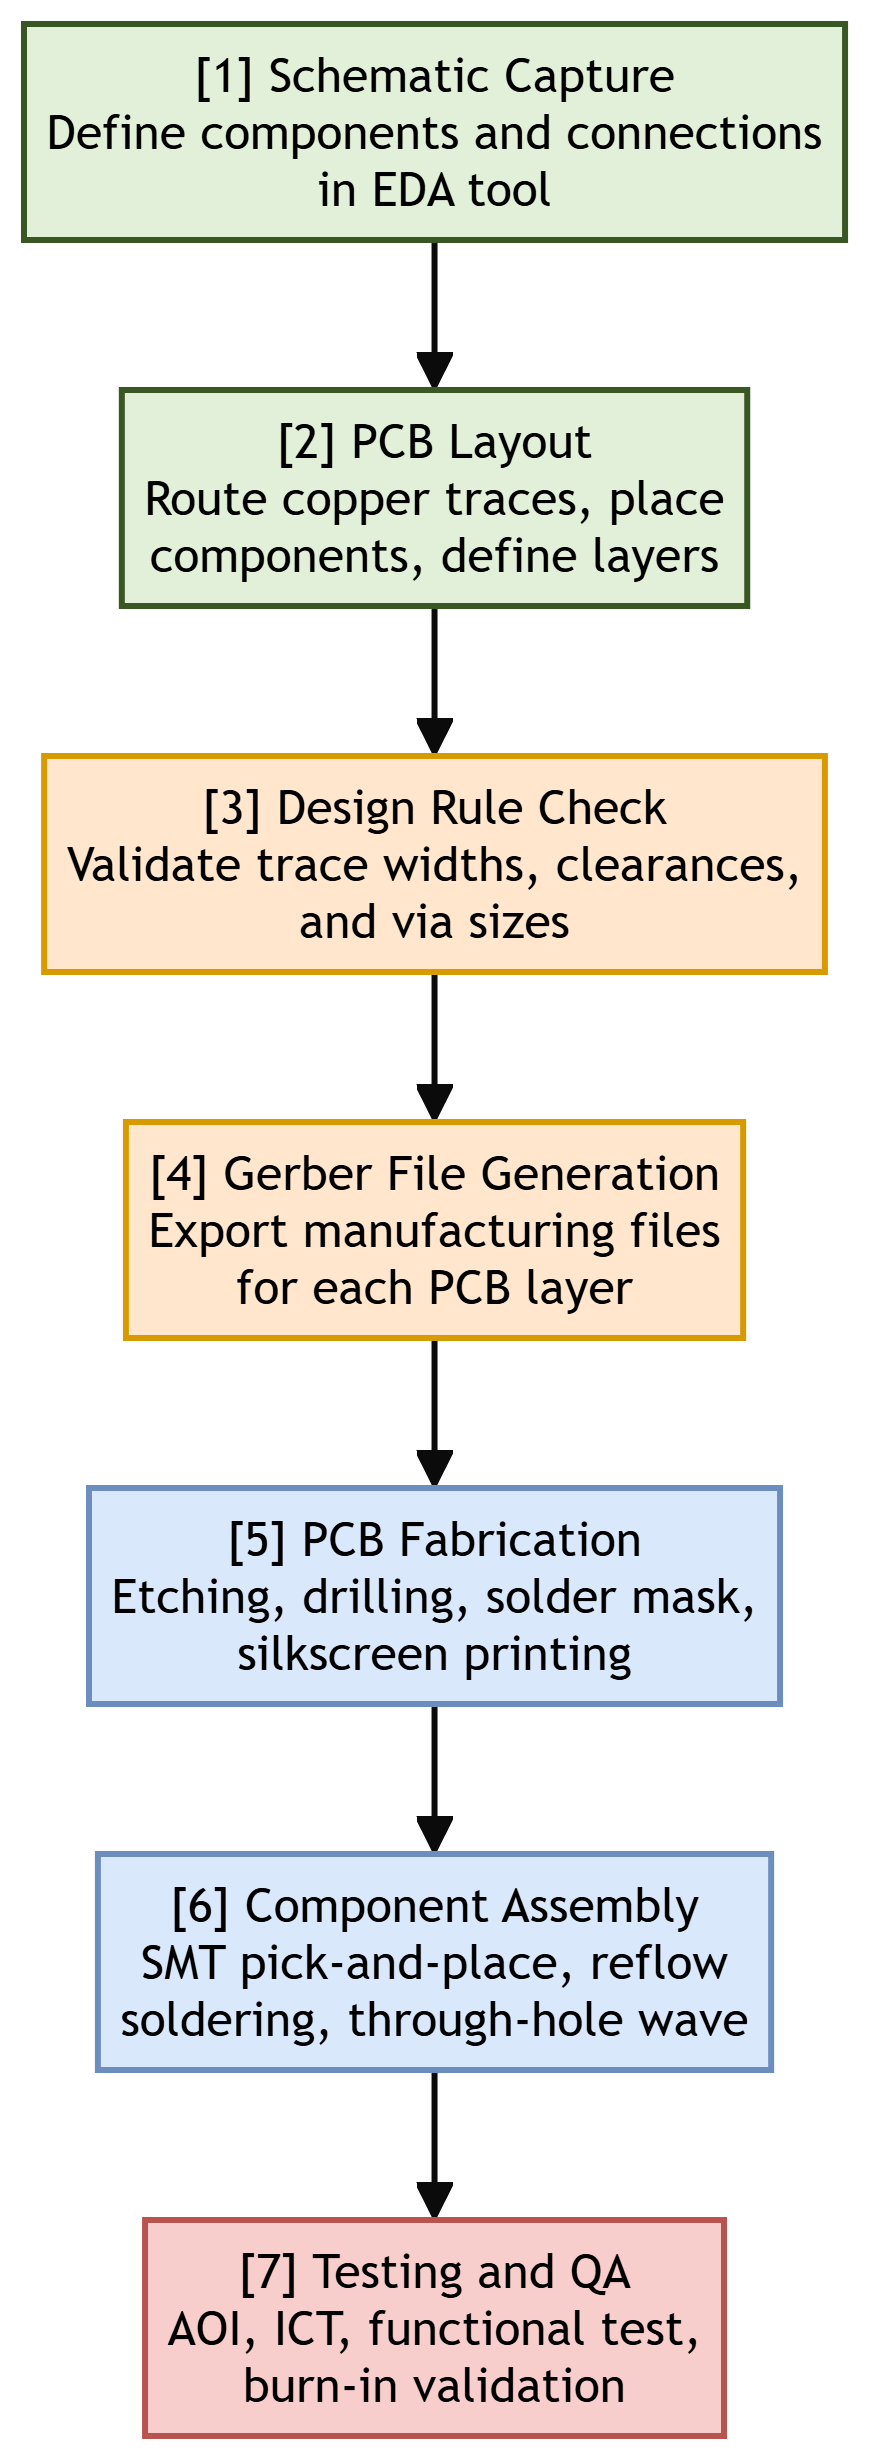
\includegraphics[width=0.75\textwidth,height=0.32\textheight,keepaspectratio]{../Images/chapter_09/pcb_manufacturing_pipeline.png}
\caption{PCB Design to Mass Manufacturing Pipeline}
\end{figure}


\subsection{2. Steps in PCB Design and Manufacturing}

\subsubsection{Step 1: Schematic Capture}
\begin{itemize}
  \item   \textbf{Action:} Using an Electronic Design Automation (EDA) tool (e.g., KiCad, Altium Designer, Eagle), the engineer creates a logical circuit diagram defining all components and their electrical connections.
  \item   \textbf{Output:} A netlist file mapping every pin-to-pin connection.
\end{itemize}

\subsubsection{Step 2: PCB Layout (Board Design)}
\begin{itemize}
  \item   \textbf{Action:} The schematic netlist is imported into the PCB layout editor. The engineer places component footprints on the board and routes copper traces connecting them.
  \item   \textbf{Key Design Considerations:}
  \item   \textbf{Trace Width:} Thicker traces for high-current power paths; thinner traces for low-current signals.
  \item   \textbf{Layer Count:} Simple designs use 2-layer boards (top and bottom copper). Complex designs use 4-layer or 6-layer boards with dedicated power and ground planes for improved noise immunity.
  \item   \textbf{Component Placement:} Place decoupling capacitors as close as possible to power pins. Keep the antenna away from copper planes and metal components.
  \item   \textbf{Via Placement:} Use vias to route signals between layers. Minimize via count to reduce manufacturing cost and signal integrity loss.
\end{itemize}

\subsubsection{Step 3: Design Rule Check (DRC)}
\begin{itemize}
  \item   \textbf{Action:} The EDA tool automatically verifies that all traces meet the fabrication house's minimum specifications for trace width, clearance between traces, hole sizes, and annular ring dimensions.
  \item   \textbf{Output:} A DRC report listing any violations that must be corrected before manufacturing.
\end{itemize}

\subsubsection{Step 4: Gerber File Generation}
\begin{itemize}
  \item   \textbf{Action:} Export the final board design as Gerber files (the universal, industry-standard format). A complete Gerber set includes a separate file for each copper layer, solder mask layer, silkscreen layer, and the drill file.
  \item   \textbf{Output:} A ZIP archive of Gerber and drill files ready for submission to the PCB fabrication house.
\end{itemize}

\subsubsection{Step 5: PCB Fabrication}
\begin{itemize}
  \item   \textbf{Action:} The fabrication house receives the Gerber files and manufactures the bare PCB:
\end{itemize}
\begin{enumerate}
  \item Print the circuit pattern onto copper-clad laminate using photolithography.
  \item Etch away unwanted copper using a chemical bath (e.g., ferric chloride).
  \item Drill holes for through-hole components and vias using CNC drill machines.
  \item Apply solder mask (the green/blue/red protective coating) and silkscreen (white component labels).
  \item Apply surface finish (HASL, ENIG gold plating) to exposed copper pads.
\end{enumerate}

\subsubsection{Step 6: Component Assembly (PCB Assembly - PCBA)}
\begin{itemize}
  \item   \textbf{Action:} Electronic components are mounted and soldered onto the fabricated bare PCB:
  \item   \textbf{SMT (Surface Mount Technology):} A pick-and-place machine positions tiny SMD components. The board passes through a reflow oven to melt solder paste and bond components.
  \item   \textbf{Through-Hole (THT):} Larger connectors and heavy components are inserted through drilled holes and soldered using wave soldering or manual soldering.
\end{itemize}

\subsubsection{Step 7: Testing and Quality Assurance}
\begin{itemize}
  \item   \textbf{Action:} Each assembled board undergoes rigorous testing:
  \item   \textbf{AOI (Automated Optical Inspection):} Camera systems scan for missing components, solder bridges, and misalignment.
  \item   \textbf{ICT (In-Circuit Testing):} Electrical probes test continuity, resistance, and capacitance of individual components and connections.
  \item   \textbf{Functional Test:} The board is powered on and firmware is flashed. A test jig verifies that all sensors, communication links, and actuators function correctly.
  \item   \textbf{Burn-In Test:} Boards are operated under stress conditions (elevated temperature) for 24–72 hours to weed out early-life failures (infant mortality).
\end{itemize}


\section{Section 2: IoT System Testing Before Mass Manufacture (Q9.2) [15M]}

\subsection{1. Introduction}
Before committing to mass production, an IoT product must undergo a comprehensive, multi-layered testing regime to ensure reliability, safety, security, and user satisfaction.

\begin{figure}[H]
\centering
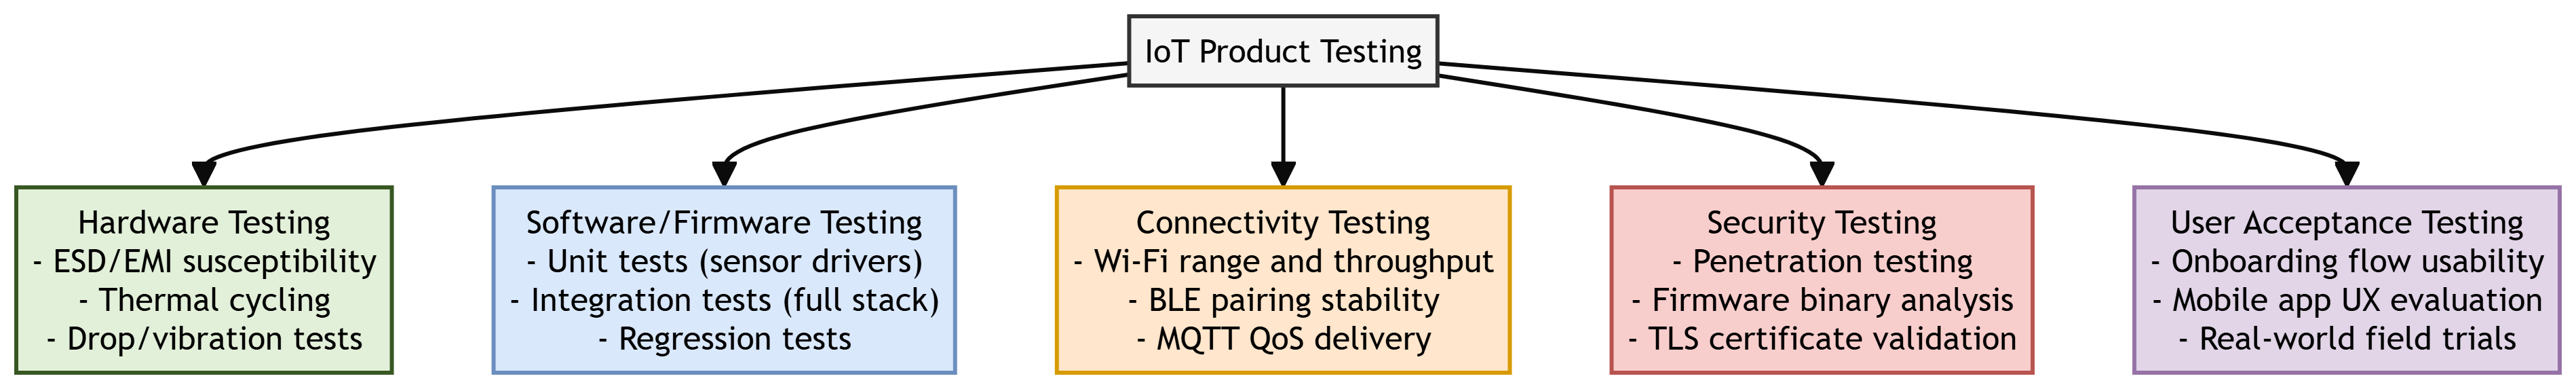
\includegraphics[width=0.75\textwidth,height=0.32\textheight,keepaspectratio]{../Images/chapter_09/iot_testing_pyramid.png}
\caption{IoT Product Testing Pyramid}
\end{figure}


\subsection{2. Five Categories of IoT System Testing}

\subsubsection{A. Hardware Testing}
\begin{itemize}
  \item   \textbf{Objective:} Verify the physical durability and electrical robustness of the device.
  \item   \textbf{Tests:}
\end{itemize}
\begin{enumerate}
  \item \textbf{ESD (Electrostatic Discharge) Testing:} Subject the device to high-voltage static discharge pulses (per IEC 61000-4-2) to ensure it survives real-world handling.
  \item \textbf{Thermal Cycling:} Repeatedly cycle the device between extreme temperatures (e.g., -20°C to +70°C) to test solder joint reliability and component tolerance.
  \item \textbf{Drop and Vibration Testing:} Drop the device from standard heights (e.g., 1.5 meters onto concrete) and subject it to sustained vibration profiles to simulate shipping and daily use.
  \item \textbf{EMI/EMC Testing:} Ensure the device does not emit excessive electromagnetic interference and operates correctly in the presence of external RF noise (per FCC Part 15 / EN 55032).
\end{enumerate}

\subsubsection{B. Software / Firmware Testing}
\begin{itemize}
  \item   \textbf{Objective:} Ensure the embedded firmware is correct, stable, and free of critical bugs.
  \item   \textbf{Tests:}
\end{itemize}
\begin{enumerate}
  \item \textbf{Unit Testing:} Test individual software modules (e.g., a single sensor driver function) in isolation.
  \item \textbf{Integration Testing:} Test the interaction between multiple modules (e.g., sensor reading → data formatting → MQTT publish → cloud reception).
  \item \textbf{Regression Testing:} Re-run all existing tests after every code change to ensure new commits do not break previously working features.
  \item \textbf{OTA Update Testing:} Verify that Over-The-Air firmware updates install correctly, roll back gracefully on failure, and do not brick the device.
\end{enumerate}

\subsubsection{C. Connectivity Testing}
\begin{itemize}
  \item   \textbf{Objective:} Validate wireless communication range, stability, and data integrity.
  \item   \textbf{Tests:}
\end{itemize}
\begin{enumerate}
  \item \textbf{Wi-Fi Range and Throughput:} Measure signal strength (RSSI) and data transfer rates at increasing distances and through various obstacle types (walls, floors).
  \item \textbf{BLE Pairing Stability:} Test Bluetooth Low Energy device discovery, pairing, and data exchange across multiple smartphone models (Android and iOS).
  \item \textbf{MQTT QoS Delivery:} Verify that messages published at QoS 1 and QoS 2 are reliably delivered even during intermittent network outages and reconnections.
\end{enumerate}

\subsubsection{D. Security Testing}
\begin{itemize}
  \item   \textbf{Objective:} Identify and remediate vulnerabilities before deployment.
  \item   \textbf{Tests:}
\end{itemize}
\begin{enumerate}
  \item \textbf{Penetration Testing:} Ethical hackers attempt to compromise the device via network attacks, API abuse, and physical tampering.
  \item \textbf{Firmware Binary Analysis:} Extract and decompile the firmware binary to check for hardcoded credentials, API keys, and unencrypted sensitive data.
  \item \textbf{TLS/SSL Certificate Validation:} Confirm that the device correctly validates server certificates and rejects expired or self-signed certificates.
  \item \textbf{Secure Boot Verification:} Ensure the bootloader only executes cryptographically signed firmware images.
\end{enumerate}

\subsubsection{E. User Acceptance Testing (UAT)}
\begin{itemize}
  \item   \textbf{Objective:} Validate the complete end-to-end user experience.
  \item   \textbf{Tests:}
\end{itemize}
\begin{enumerate}
  \item \textbf{Onboarding Flow:} Test the first-time setup experience (unboxing → Wi-Fi provisioning → account creation → first data reading) across diverse user demographics.
  \item \textbf{Mobile App UX:} Evaluate the companion mobile app for responsiveness, intuitiveness, and error handling.
  \item \textbf{Real-World Field Trials:} Deploy 50–100 units to beta testers in actual home/office/industrial environments for 2–4 weeks and collect usage logs, crash reports, and qualitative feedback.
\end{enumerate}


\section{Section 3: Scaling from Prototype to Manufacture (Q9.3) [10M]}

\subsection{1. Designing Kits}
\begin{itemize}
  \item   Before full mass production, many IoT startups release a \textbf{developer kit} — a small-batch, semi-assembled product sold to early adopters and partner developers.
  \item   \textbf{Purpose:} Validates the supply chain, tests assembly procedures, and generates early revenue and community feedback.
  \item   \textbf{Contents:} The PCB, pre-programmed firmware, an enclosure, mounting hardware, cables, and a quick-start guide.
\end{itemize}


\subsection{2. Mass-Producing the Case and Fixtures (Injection Molding)}
\begin{itemize}
  \item   \textbf{Process:} Molten plastic (e.g., ABS, Polycarbonate) is injected at high pressure into a precision-machined steel mold cavity. After cooling, the mold opens and the solid plastic part is ejected.
  \item   \textbf{Advantages:} Produces thousands of identical, smooth, production-quality enclosures per day at very low per-unit cost (often $<$ \$0.50/unit at scale).
  \item   \textbf{Disadvantages:} Extremely high upfront tooling cost (\$10,000–\$100,000+ for steel molds). Any design change after mold fabrication requires a new mold.
  \item   \textbf{Design Constraints:} Parts must have draft angles (tapered walls) for easy ejection, uniform wall thickness to prevent warping, and rounded internal corners to avoid stress concentrations.
\end{itemize}


\subsection{3. Obtaining Certifications}
Before an IoT product can be legally sold in a target market, it must obtain regulatory certifications:

\begin{table}[H]
\centering
\begin{tabular}{|p{\dimexpr 0.2\textwidth - 2\tabcolsep - 1.5\arrayrulewidth\relax}|p{\dimexpr 0.4\textwidth - 2\tabcolsep - 1.5\arrayrulewidth\relax}|p{\dimexpr 0.4\textwidth - 2\tabcolsep - 1.5\arrayrulewidth\relax}|}
\hline
Certification & Region & Scope \\
\hline
\textbf{FCC Part 15} & United States & Limits unintentional RF emissions from electronic devices. \\
\hline
\textbf{CE Marking} & European Union & Declares conformity with EU health, safety, and environmental directives. \\
\hline
\textbf{RoHS} & EU / Global & Restricts use of hazardous substances (lead, mercury, cadmium) in electronics. \\
\hline
\textbf{UL / IEC 62368-1} & Global & Electrical safety certification for audio/video and IT equipment. \\
\hline
\textbf{IC} & Canada & Radio equipment certification (equivalent to FCC). \\
\hline
\end{tabular}
\end{table}

\begin{itemize}
  \item   \textbf{Process:} Submit production samples and technical documentation to an accredited testing laboratory. Testing typically takes 4–8 weeks and costs \$5,000–\$30,000 depending on the number of radio interfaces.
\end{itemize}


\subsection{4. Scaling Up Software}
\begin{itemize}
  \item   \textbf{Cloud Infrastructure Scaling:} Move from a single development server to auto-scaling cloud infrastructure (e.g., AWS ECS, Kubernetes) capable of handling millions of concurrent device connections.
  \item   \textbf{Device Fleet Management:} Implement centralized dashboards for monitoring device health, managing firmware versions, and performing bulk OTA updates across thousands of deployed devices.
  \item   \textbf{Database Scaling:} Transition from a single relational database to distributed NoSQL or time-series databases (e.g., InfluxDB, TimescaleDB, DynamoDB) designed for high-velocity IoT data ingestion.
  \item   \textbf{CI/CD Pipelines:} Establish continuous integration and continuous deployment pipelines for firmware and cloud services to enable rapid, tested, and automated releases.
\end{itemize}
